\documentclass{ximera}

\usepackage{epsfig}

\graphicspath{
  {./}
  {figures/}
}


\usepackage{morewrites}

%\newcounter{ccounter}
%\setcounter{ccounter}{1}
%\newcommand{\Chapter}[1]{\setcounter{chapter}{\arabic{ccounter}}\chapter{#1}\addtocounter{ccounter}{1}}

%\newcommand{\section}[1]{\section{#1}\setcounter{thm}{0}\setcounter{equation}{0}}

%\renewcommand{\theequation}{\arabic{chapter}.\arabic{section}.\arabic{equation}}
%\renewcommand{\thefigure}{\arabic{chapter}.\arabic{figure}}
%\renewcommand{\thetable}{\arabic{chapter}.\arabic{table}}

%\newcommand{\Sec}[2]{\section{#1}\markright{\arabic{ccounter}.\arabic{section}.#2}\setcounter{equation}{0}\setcounter{thm}{0}\setcounter{figure}{0}}

\newcommand{\Sec}[2]{\section{#1}}

\setcounter{secnumdepth}{2}
%\setcounter{secnumdepth}{1} 

%\newcounter{THM}
%\renewcommand{\theTHM}{\arabic{chapter}.\arabic{section}}

\newcommand{\trademark}{{R\!\!\!\!\!\bigcirc}}
%\newtheorem{exercise}{}

\newcommand{\dfield}{{\sf dfield9}}
\newcommand{\pplane}{{\sf pplane9}}

\newcommand{\EXER}{\section*{Exercises}}%\vspace*{0.2in}\hrule\small\setcounter{exercise}{0}}
\newcommand{\CEXER}{}%\vspace{0.08in}\begin{center}Computer Exercises\end{center}}
\newcommand{\TEXER}{} %\vspace{0.08in}\begin{center}Hand Exercises\end{center}}
\newcommand{\AEXER}{} %\vspace{0.08in}\begin{center}Hand Exercises\end{center}}

% BADBAD: \newcommand{\Bbb}{\bf}

\newcommand{\R}{\mbox{$\Bbb{R}$}}
\newcommand{\C}{\mbox{$\Bbb{C}$}}
\newcommand{\Z}{\mbox{$\Bbb{Z}$}}
\newcommand{\N}{\mbox{$\Bbb{N}$}}
\newcommand{\D}{\mbox{{\bf D}}}
\usepackage{amssymb}
%\newcommand{\qed}{\hfill\mbox{\raggedright$\square$} \vspace{1ex}}
%\newcommand{\proof}{\noindent {\bf Proof:} \hspace{0.1in}}

\newcommand{\setmin}{\;\mbox{--}\;}
\newcommand{\Matlab}{{M\small{AT\-LAB}} }
\newcommand{\Matlabp}{{M\small{AT\-LAB}}}
\newcommand{\computer}{\Matlab Instructions}
\newcommand{\half}{\mbox{$\frac{1}{2}$}}
\newcommand{\compose}{\raisebox{.15ex}{\mbox{{\scriptsize$\circ$}}}}
\newcommand{\AND}{\quad\mbox{and}\quad}
\newcommand{\vect}[2]{\left(\begin{array}{c} #1_1 \\ \vdots \\
 #1_{#2}\end{array}\right)}
\newcommand{\mattwo}[4]{\left(\begin{array}{rr} #1 & #2\\ #3
&#4\end{array}\right)}
\newcommand{\mattwoc}[4]{\left(\begin{array}{cc} #1 & #2\\ #3
&#4\end{array}\right)}
\newcommand{\vectwo}[2]{\left(\begin{array}{r} #1 \\ #2\end{array}\right)}
\newcommand{\vectwoc}[2]{\left(\begin{array}{c} #1 \\ #2\end{array}\right)}



\newcommand{\inv}{^{-1}}
\newcommand{\CC}{{\cal C}}
\newcommand{\CCone}{\CC^1}
\newcommand{\Span}{{\rm span}}
\newcommand{\rank}{{\rm rank}}
\newcommand{\trace}{{\rm tr}}
\newcommand{\RE}{{\rm Re}}
\newcommand{\IM}{{\rm Im}}
\newcommand{\nulls}{{\rm null\;space}}

\newcommand{\dps}{\displaystyle}
\newcommand{\arraystart}{\renewcommand{\arraystretch}{1.8}}
\newcommand{\arrayfinish}{\renewcommand{\arraystretch}{1.2}}
\newcommand{\Start}[1]{\vspace{0.08in}\noindent {\bf Section~\ref{#1}}}
\newcommand{\exer}[1]{\noindent {\bf \ref{#1}}}
\newcommand{\ans}{}
\newcommand{\matthree}[9]{\left(\begin{array}{rrr} #1 & #2 & #3 \\ #4 & #5 & #6
\\ #7 & #8 & #9\end{array}\right)}
\newcommand{\cvectwo}[2]{\left(\begin{array}{c} #1 \\ #2\end{array}\right)}
\newcommand{\cmatthree}[9]{\left(\begin{array}{ccc} #1 & #2 & #3 \\ #4 & #5 &
#6 \\ #7 & #8 & #9\end{array}\right)}
\newcommand{\vecthree}[3]{\left(\begin{array}{r} #1 \\ #2 \\
#3\end{array}\right)}
\newcommand{\cvecthree}[3]{\left(\begin{array}{c} #1 \\ #2 \\
#3\end{array}\right)}
\newcommand{\cmattwo}[4]{\left(\begin{array}{cc} #1 & #2\\ #3
&#4\end{array}\right)}

\newcommand{\Matrix}[1]{\ensuremath{\left(\begin{array}{rrrrrrrrrrrrrrrrrr} #1 \end{array}\right)}}

\newcommand{\Matrixc}[1]{\ensuremath{\left(\begin{array}{cccccccccccc} #1 \end{array}\right)}}



\renewcommand{\labelenumi}{\theenumi)}
\newenvironment{enumeratea}%
{\begingroup
 \renewcommand{\theenumi}{\alph{enumi}}
 \renewcommand{\labelenumi}{(\theenumi)}
 \begin{enumerate}}
 {\end{enumerate}\endgroup}



\newcounter{help}
\renewcommand{\thehelp}{\thesection.\arabic{equation}}

%\newenvironment{equation*}%
%{\renewcommand\endequation{\eqno (\theequation)* $$}%
%   \begin{equation}}%
%   {\end{equation}\renewcommand\endequation{\eqno \@eqnnum
%$$\global\@ignoretrue}}

%\input{psfig.tex}

\author{Martin Golubitsky and Michael Dellnitz}

%\newenvironment{matlabEquation}%
%{\renewcommand\endequation{\eqno (\theequation*) $$}%
%   \begin{equation}}%
%   {\end{equation}\renewcommand\endequation{\eqno \@eqnnum
% $$\global\@ignoretrue}}

\newcommand{\soln}{\textbf{Solution:} }
\newcommand{\exercap}[1]{\centerline{Figure~\ref{#1}}}
\newcommand{\exercaptwo}[1]{\centerline{Figure~\ref{#1}a\hspace{2.1in}
Figure~\ref{#1}b}}
\newcommand{\exercapthree}[1]{\centerline{Figure~\ref{#1}a\hspace{1.2in}
Figure~\ref{#1}b\hspace{1.2in}Figure~\ref{#1}c}}
\newcommand{\para}{\hspace{0.4in}}

\renewenvironment{solution}{\suppress}{\endsuppress}

\ifxake
\newenvironment{matlabEquation}{\begin{equation}}{\end{equation}}
\else
\newenvironment{matlabEquation}%
{\let\oldtheequation\theequation\renewcommand{\theequation}{\oldtheequation*}\begin{equation}}%
  {\end{equation}\let\theequation\oldtheequation}
\fi

\makeatother


\title{Linear Systems in Jordan Normal Form}

\begin{document}
\begin{abstract}
\end{abstract}
\maketitle


\label{sec:LinHomSys}

In this section we discuss one method for finding 
closed form solutions\index{closed form solution} to 
linear constant coefficient systems of ODEs based on 
Jordan normal form\index{Jordan normal form}. Let  
\begin{equation}  \label{eq:linsys}
\dps\frac{dX}{dt} = AX,
\end{equation}
where $A=(a_{ij})$ is a constant $n\times n$ matrix and $X$ is an 
$n$ vector.  In Theorem~\ref{T:linODEsoln} of Chapter~\ref{Chap:Planar} 
we showed that the general solution\index{general solution} to 
\eqref{eq:linsys} is
\[
X(t) = e^{tA}X_0,
\]
where $X_0=X(0)$ is the initial condition\index{initial condition}.  
In Chapter~\ref{Chap:Planar} 
we used this theorem to solve planar systems of ODEs in closed form.
Now we apply matrix exponentials to solve \eqref{eq:linsys} for an 
arbitrary matrix $A$ --- at least in principle.
There were three ideas behind finding solutions to planar systems:
\begin{itemize}
\item[(a)] Exponentials\index{matrix!exponential} of similar 
matrices are similar\index{similar}.  More precisely,
\[
e^{P\inv AP} = P\inv e^{A}P,
\]
where $P$ is any invertible\index{invertible} matrix.  
See Chapter~\ref{Chap:Planar}, Lemma~\ref{L:similarexp}.
\item[(b)]	Every matrix $A$ is similar to a matrix in Jordan normal 
form --- in two dimensions the Jordan normal forms are
\[
B_1=\mattwo{\lambda}{0}{0}{\mu}, \quad B_2=\mattwo{\sigma}{-\tau}{\tau}{\sigma}
\AND B_3=\mattwo{\lambda}{1}{0}{\lambda}
\]
The first matrix corresponds to two 
real eigenvalues\index{eigenvalue!real} $\lambda$, $\mu$
with linearly independent eigenvectors; the second matrix 
corresponds to complex eigenvalues\index{eigenvalue!complex} 
$\sigma\pm i\tau$; and the third matrix is the only nontrivial 
Jordan block\index{Jordan block} in two dimensions.
\item[(c)]	It is possible to compute the exponentials of matrices in
Jordan normal form\index{Jordan normal form}.  Indeed,
\begin{eqnarray*}
e^{tB_1} &  = & \mattwo{e^{\lambda t}}{0}{0}{e^{\mu t}} \\
e^{tB_2} & = & 
e^{\sigma t}\mattwo{\cos(\tau t)}{-\sin(\tau t)}{\sin(\tau t)}{\cos(\tau t)} \\
e^{tB_3} & = &  e^{\lambda t}\mattwo{1}{t}{0}{1}.
\end{eqnarray*}
\end{itemize}

We use the same approach for solving linear systems in higher dimensions.
But in order to compute exponentials of matrices in Jordan normal form,
we need to verify one additional remark.

\begin{lemma}  \label{T:blocks}
Let the matrix $A$ be block diagonal, that is, let
\[
A=\mattwo{C_1}{0}{0}{C_2},
\]
where $C_1$ is a $\ell\times \ell$ matrix and $C_2$ is an 
$(n-\ell)\times(n-\ell)$ matrix.  Then 
\[
e^A = \mattwo{e^{C_1}}{0}{0}{e^{C_2}}.
\]
\end{lemma}

\begin{proof}  This lemma is proved by noting that
\[
A^k = \mattwo{C_1^k}{0}{0}{C_2^k},
\]
and applying the power series definition of matrix exponential.  
See Chapter~\ref{Chap:Planar}, \eqref{e:expL}. \end{proof}

\subsection*{Matrix Exponentials of Jordan Normal Forms}

We compute matrix exponentials in two steps: first we consider 
Jordan blocks corresponding to real eigenvalues and second we consider
Jordan blocks with complex eigenvalues.  In this section we discuss mainly
solutions to linear systems already in Jordan normal form.  That is, we 
assume that a similarity transformation has already been performed that put
the coefficient
matrix into Jordan normal form.  In the next chapter, Section~\ref{S:SEOC},
we consider solving linear systems in their original coordinates. 

\subsection*{Real Eigenvalues}

A Jordan block with a real simple eigenvalue is just a $1\times 1$ matrix
$(\lambda)$. This matrix corresponds to the single equation 
$\dot{x}=\lambda x$ whose solution is $x(t) = e^{\lambda t}x_0$.

The $k\times k$ Jordan block\index{Jordan block} with real 
eigenvalue\index{Jordan block!with real eigenvalue} $\lambda$ is 
\[
\lambda I_k + N
\]
where the only nonzero entries in $N$ are the $1$s on the superdiagonal.  
Recall that \eqref{e:Ndef} in Chapter~\ref{C:HDeigenvalues} implies that 
$N^k=0$.  Since $I_k$ and $N$ commute, Proposition~\ref{P:expAB} of 
Chapter~\ref{Chap:Planar} implies that $e^{t(I_n+N)}=e^{tI_n}e^{tN}$.  We 
can compute the solution to the differential equation as:
\begin{eqnarray}
X(t) & = & e^{\lambda t}e^{tN}X_0 \nonumber \\
& = & e^{\lambda t}\left(I_k+tN+\cdots+\frac{1}{k!}t^{k-1}N^{k-1}\right)X_0.
\label{e:expsoln}
\end{eqnarray}

Note that $N^2$ is the matrix with $1$s on the second diagonal above the main
diagonal and $0$s elsewhere.  Similarly, $N^3$ is the matrix with $1$s on the 
third diagonal above the main diagonal and $0$s elsewhere, etc.
 

\subsubsection*{An Example of a Real Eigenvalue Jordan Block Equation}

Consider the case of a $k=3$ Jordan block with eigenvalue $\lambda=-0.5$.  
Then
\[
X(t) = e^{-0.5t} \left(\begin{array}{ccc} 1 & t & \frac{t^2}{2} \\
0 & 1 & t \\ 0 & 0 & 1 \end{array}\right)X_0.
\]
We can now solve the initial value problem\index{initial value problem}
\index{closed form solution} in closed form.  For example,
suppose $X_0=(0.5,1.5,2)$, and let $X(t)=(x_1(t),x_2(t),x_3(t))$.  Then 
the solution of this initial value problem is:
\begin{equation}  \label{E:x1examp}
\begin{array}{rcl}
x_1(t) & = & e^{-0.5t}(0.5 + 1.5t + t^2) \\
x_2(t) & = & e^{-0.5t}(1.5 + 2t) \\
x_3(t) & = & 2e^{-0.5t}.
\end{array}
\end{equation}
In Figure~\ref{F:Jordan} we graph the time series for $x_1$ as a
function of $t$.  Note the initial growth in $x_1$ (due to the quadratic 
polynomial factor in $x_1$) before exponential decay\index{exponential!decay} 
dominates the quadratic growth.  See Exercise~\ref{c11.1.4}.

\begin{figure}[htb]
     \centerline{%
     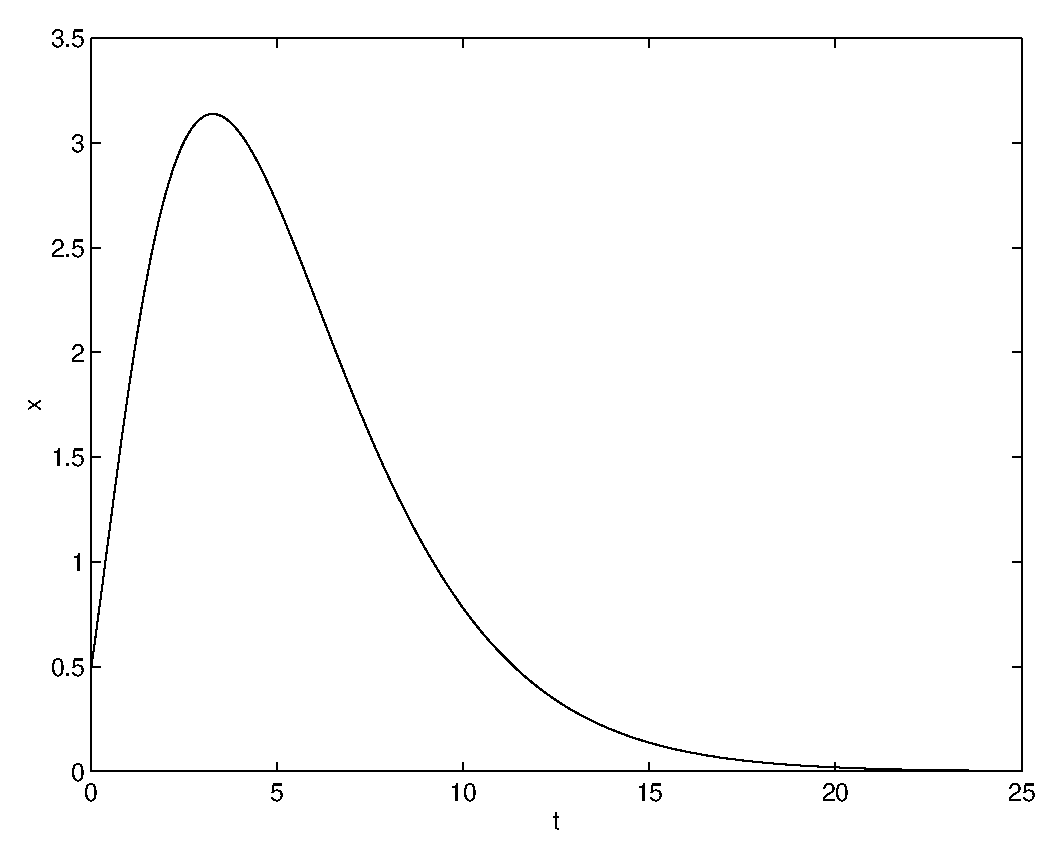
\psfig{file=../figures/jordan.eps,width=3.5in}}
     \caption{First component $x_1(t)$ of solution to
	Jordan block equation for $k=3$ when $X(0)=(0.5,1.5,2)$.}
     \label{F:Jordan}
\end{figure}

\subsection*{Complex Eigenvalues}
\index{Jordan block}\index{Jordan block!with complex eigenvalue}

If $A$ is the Jordan block corresponding to a simple complex eigenvalue
$\lambda=\sigma+i\tau$, then \eqref{eq:linsys} is the two dimensional system 
\[
\frac{dX}{dt}=\mattwo{\sigma}{-\tau}{\tau}{\sigma} X
\]
whose solutions have the form 
\[
X(t)=e^{\sigma t}\mattwo{\cos(\tau t)}{-\sin(\tau t)} 
{\sin(\tau t)}{\cos(\tau t)} X_0.
\]

The general Jordan block corresponding to a multiplicity $k$ complex
eigenvalue $\sigma+i\tau$ has the form 
\begin{equation} \label{e:JM}
J + M
\end{equation}
where $J$ is a block diagonal\index{matrix!block diagonal} 
$2k\times 2k$ matrix with $k$ identical $2\times 2$ matrices 
\[
\mattwo{\sigma}{-\tau}{\tau}{\sigma}
\]
on the diagonal and $M$ is a $2k\times 2k$ block form matrix 
whose nonzero blocks have $I_2$ on the superdiagonal.

Since $J$ and $M$ commute, Proposition~\ref{P:expAB} of 
Chapter~\ref{Chap:Planar} implies that
\[
e^{t(J+M)} = e^{tJ} e^{tM}.
\]
As in the case of real eigenvalues $M^k=0$.  Now since $tJ$ is block 
diagonal, we can use Lemma~\ref{T:blocks} to determine that $e^{tJ}$ 
is also block diagonal with blocks 
\[
e^{\sigma t}\mattwo{\cos(\tau t)}{-\sin(\tau t)}{\sin(\tau t)}{\cos(\tau t)}.
\]
Putting these two observations together allows us to solve explicitly 
ODE systems whose coefficient matrix\index{matrix!coefficient}
is a single Jordan block\index{Jordan block} with complex eigenvalues.



\subsubsection*{An Example of a Complex Eigenvalue Jordan Block Equation}

Find the solution to the differential equation 
\[
\frac{dX}{dt} = \left(\begin{array}{rr|rr|rr} 
 2 & 1 & 1 & 0 & 0 & 0\\
-1 & 2 & 0 & 1 & 0 & 0 \\  
 \hline
 0 & 0 & 2 & 1 & 1 & 0 \\
 0 & 0 &-1 & 2 & 0 & 1 \\
\hline
 0 & 0 & 0 & 0 & 2 & 1\\
 0 & 0 & 0 & 0 &-1 & 2  \end{array}\right) X
\]
with initial condition
\[
X_0 = (1, 3, -2, 0, 0, 4).
\]

Using the notation of \eqref{e:JM} we have
\[
J = \left(\begin{array}{rr|rr|rr} 
 2 & 1 & 0 & 0 & 0 & 0\\
-1 & 2 & 0 & 0 & 0 & 0 \\  
 \hline
 0 & 0 & 2 & 1 & 0 & 0 \\
 0 & 0 &-1 & 2 & 0 & 0 \\
\hline
 0 & 0 & 0 & 0 & 2 & 1\\
 0 & 0 & 0 & 0 &-1 & 2  \end{array}\right) 
\AND 
M = \left(\begin{array}{rr|rr|rr} 
 0 & 0 & 1 & 0 & 0 & 0\\
0 & 0 & 0 & 1 & 0 & 0 \\  
 \hline
 0 & 0 & 0 & 0 & 1 & 0 \\
 0 & 0 & 0 & 0 & 0 & 1 \\
\hline
 0 & 0 & 0 & 0 & 0 & 0\\
 0 & 0 & 0 & 0 & 0 & 0  \end{array}\right).
\]
It follows that 
\begin{eqnarray*}
X(t) & = & e^{tJ}e^{tM}X_0 \\
 & = & e^{2t}\left(\begin{array}{rr|rr|rr} 
 \cos t & -\sin t & 0 & 0 & 0 & 0\\
\sin t & \cos t & 0 & 0 & 0 & 0 \\  
 \hline
 0 & 0 & \cos t & -\sin t & 0 & 0 \\
 0 & 0 & \sin t & \cos t & 0 & 0 \\
\hline
 0 & 0 & 0 & 0 & \cos t & -\sin t\\
 0 & 0 & 0 & 0 & \sin t & \cos t  \end{array}\right) 
\left(\begin{array}{rr|rr|rr} 
 1 & 0 & t & 0 & \half t^2 & 0\\
0 & 1 & 0 & t & 0 & \half t^2 \\  
 \hline
 0 & 0 & 1 & 0 & t & 0 \\
 0 & 0 & 0 & 1 & 0 & t \\
\hline
 0 & 0 & 0 & 0 & 1 & 0\\
 0 & 0 & 0 & 0 & 0 & 1  \end{array}\right) X_0 \\
 & = & e^{2t}\left(\begin{array}{rr|rr|rr} 
 \cos t & -\sin t & t\cos t & -t\sin t & \half t^2\cos t & -\half t^2\sin t\\
\sin t & \cos t & t\sin t & t\cos t & \half t^2\sin t & \half t^2\cos t \\  
 \hline
 0 & 0 & \cos t & -\sin t & t\cos t & -t\sin t \\
 0 & 0 & \sin t & \cos t & t\sin t & t\cos t \\
\hline
 0 & 0 & 0 & 0 & \cos t & -\sin t\\
 0 & 0 & 0 & 0 & \sin t & \cos t  \end{array}\right)
\left(\begin{array}{r} 1 \\ 3 \\ \hline -2 \\  0 \\ \hline 0 \\ 4
\end{array}\right).
\end{eqnarray*}
Finally,
\[
X(t) = e^{2t}\left(\begin{array}{c}
\cos t - 3\sin t -2t\cos t - 2t^2\sin t \\
\sin t + 3\cos t -2t\sin t + 2t^2\cos t \\
-2\cos t - 4t\sin t \\
-2\sin t + 4t\cos t \\
-4\sin t \\ 4\cos t \end{array}\right).
\]
Moreover, this example is typical of all such Jordan block equations. 

\subsection*{Solutions When Matrices are Not in Jordan Normal Form} 

Let $A$ and $B=S\inv AS$ be similar $n\times n$ matrices.  Recall 
Lemma~\ref{L:simsoln} of Chapter~\ref{Chap:Planar} which states that 
$X(t)=SY(t)$ is a solution to $\dot{X}=AX$ if and only if $Y(t)$ is a 
solution to
\begin{equation} \label{E:JNFDE}
\frac{dY}{dt} = BY.
\end{equation}

Suppose that $B$ is in Jordan normal form; then we know how to solve 
\eqref{E:JNFDE} using matrix exponentials and can then solve the original
equation $\dot{X}=AX$ in principle by multiplying $Y(t)$ by $S$.  This 
approach is clean in theory, but messy in practice.  

As an example, consider the differential equation $\dot{X}=AX$ where
\begin{matlabEquation}\label{MATLAB:44}
A = \left(\begin{array}{rrrr} 12 & 4 & 3 & 6 \\ 5 & 22 & 6 & -6\\
-34 & -69 & -22 & 7\\ -5 & 16 & 3 & -10 \end{array}\right),
\end{matlabEquation}
with initial condition $X_0=(1,-1,0,1)^t$.  Use {\tt eig(A)} in \Matlab to 
verify that the eigenvalues of $A$ are $-1,-1,2,2$.  Since the nullities of 
$A+I_n$ and $A-2I_n$ both equal $1$, it follows that both double eigenvalues
have nontrivial Jordan blocks, and
\[
B = \mattwoc{\mattwo{-1}{1}{0}{-1}}{0}{0}{\mattwo{2}{1}{0}{2}}
\]
is the Jordan normal form of $A$.  As noted previously, we can solve 
\eqref{E:JNFDE} using matrix exponentials, obtaining
\[
Y(t) =
\mattwoc{e^{-t}\mattwo{1}{t}{0}{1}}{0}{0}{e^{2t}\mattwo{1}{t}{0}{1}}Y_0.
\]
To find a formula for $X(t)$ we need to find the matrix $S$ such that 
$B=S\inv AS$.  Then $X(t)=SY(t)$ where $Y_0=S\inv X_0$.  Using \Matlab we
can find vectors 
\begin{eqnarray*}
v_2 & \in & \nulls((A+I_n)^2)\setmin\nulls(A+I_n) \\
v_4 & \in & \nulls((A-2I_n)^2)\setmin\nulls(A-2I_n)
\end{eqnarray*}
Then set $v_1=(A+I_n)v_2$, $v_3=(A-2I_n)v_4$ and $S=(v_1|v_2|v_3|v_4)$. 
Indeed, 
\begin{verbatim}
S =
   -0.3580   -0.1181    0.2039   -0.0775
    0.3580   -0.2399    0.1019   -0.2936
   -0.3580    0.9559   -0.6116    0.9459
    0.7160   -0.1218   -0.1019   -0.1142
\end{verbatim}
and 
\begin{verbatim}
Y0 =
    5.5285
  -16.7608
   16.0879
   29.4307
\end{verbatim}
So 
\begin{equation}  \label{E:solvedebf}
X(t) = S\mattwoc{e^{-t}\mattwo{1}{t}{0}{1}}{0}{0}{e^{2t}\mattwo{1}{t}{0}{1}}
\left(\begin{array}{r} 5.5285 \\  -16.7608 \\ 16.0879 \\ 29.4307\end{array}
\right).
\end{equation}

\subsubsection*{The General Functional Form of Solutions}

The previous calculations suggest how to prove the following lemma.

\begin{lemma}  \label{R:pdeg}
Components of solutions to the system of differential equations $\dot{X}=AX$ 
where $A$ is an $n\times n$ matrix are linear combinations of the functions 
$t^je^{\lambda t}$ where $\lambda$ is a real eigenvalue of $A$ and 
$t^je^{\sigma t}\cos(\tau t)$ and $t^je^{\sigma t}\sin(\tau t)$ where
$\sigma\pm i\tau$ is a complex eigenvalue of $A$.   The exponent $j\leq k$, 
where $k$ is the size of the largest Jordan block associated to the given
eigenvalue. 
\end{lemma}

\begin{proof}  Formula \eqref{e:expsoln} verifies this statement when $A$ is in Jordan 
normal form with real eigenvalues.  A similar formula holds with $J$ and $M$ 
when $A$ has complex eigenvalues.  Solutions to the general matrix equation 
are just linear combinations of solutions to the corresponding Jordan normal 
form equations.  Indeed, as noted in the discussion leading to \eqref{E:JNFDE}, 
solutions to the general system equation are obtained from the Jordan normal 
form equations by multiplying these special solutions by the constant matrix
$S$.  This multiplication does not alter the statement that the coordinate
functions are linear combinations of the given functions.  \end{proof}

In Section~\ref{S:SEOC} we discuss alternative methods for finding solutions 
to systems of constant coefficient linear differential equations.  All of
these methods require some effort to carry out by hand.


\EXER

\TEXER

\begin{exercise} \label{c11.1.1}
Find the solution to the system
\begin{eqnarray*}
\dot{x}_1 & = & 2x_1+x_2 \\
\dot{x}_2 & = & 2x_2 \\
\dot{x}_3 & = & x_3-x_4 \\
\dot{x}_4 & = & x_3+x_4
\end{eqnarray*}
satisfying $X_0=(-1,1,2,-3)^t$.

\begin{solution}
\ans 
\[
X(t) =
\left(\begin{array}{c}
e^{2t}(t - 1) \\
e^{2t} \\
e^t(2\cos{t} + 3\sin{t}) \\
e^t(2\sin{t} - 3\cos{t})
\end{array}\right).
\]

\soln Write the system as the equation $\dot{X} = AX$, where
\[
A =
\left(\begin{array}{rrrr}
2 & 1 & 0 & 0 \\
0 & 2 & 0 & 0 \\
0 & 0 & 1 & -1 \\
0 & 0 & 1 & 1
\end{array}\right).
\]
Note that the matrix $A$ is in Jordan normal form, and has a double
eigenvalue at $\lambda = 2$ and a pair of complex conjugate eigenvalues
at $\lambda = 1 \pm i$.  Thus, we can compute the closed form solution
$X(t) = e^{At}X_0$ by computing the exponential of each Jordan block.  Let
\[
B = \mattwo{2}{1}{0}{2} \AND C = \mattwo{1}{-1}{1}{1}.
\]
Then, $B = 2I_2 + N$, where $N$ is the $2 \times 2$ matrix with an entry $1$
on the superdiagonal.  Since $I_2$ and $N$ commute,
\[
e^{Bt} = e^{2t}e^{tN} = e^{2t}(I_2 + tN) =
e^{2t}\mattwo{1}{t}{0}{1}.
\]
Since $C$ is a $2 \times 2$ block with complex eigenvalues, we can
compute its exponential as we have done in previous chapters, using
$\sigma = 1$ and $\tau = 1$:
\[
e^{Ct} = e^{\sigma t}\mattwo{\cos{(\tau t)}}{-\sin{(\tau t)}}
{\sin{(\tau t)}}{\cos{(\tau t)}}
= e^{t}\mattwo{\cos{t}}{-\sin{t}}{\sin{t}}{\cos{t}}.
\]
Thus,
\[
X(t) = e^{At}X_0 =
\left(\begin{array}{cccc}
e^{2t} & te^{2t} & 0 & 0 \\
0 & e^{2t} & 0 & 0 \\
0 & 0 & e^t\cos{t} & -e^t\sin{t} \\
0 & 0 & e^t\sin{t} & e^t\cos{t}
\end{array}\right)
\left(\begin{array}{r} -1 \\ 1 \\ 2 \\ -3 \end{array}\right)
= \left(\begin{array}{c}
e^{2t}(t - 1) \\
e^{2t} \\
e^t(2\cos{t} + 3\sin{t}) \\
e^t(2\sin{t} - 3\cos{t})
\end{array}\right).
\]

\end{solution}
\end{exercise}

\begin{exercise} \label{c11.1.2}
Find the solution to the system
\begin{eqnarray*}
\dot{x}_1 & = & -2x_1+x_2+x_3 \\
\dot{x}_2 & = & -x_1-2x_2+x_4 \\
\dot{x}_3 & = & -2x_3+x_4 \\
\dot{x}_4 & = & -x_3-2x_4
\end{eqnarray*}
satisfying $X_0=(1,2,-1,-3)^t$.

\begin{solution}
\ans
\[
X(t) = e^{-2t}
\left(\begin{array}{c}
\cos t + 2\sin t - t(\cos t + 3\sin t) \\
2\cos t - \sin t + t(\sin t - 3\cos t) \\
-\cos t - 3\sin t \\
-\sin t - 3\cos t
\end{array}\right).
\]

\soln Write the system as $\dot{X} = AX$, where
\[
A =
\left(\begin{array}{rrrr}
-2 & 1 & 1 & 0 \\
-1 & -2 & 0 & 1 \\
0 & 0 & -2 & 1 \\
0 & 0 & -1 & -2
\end{array}\right).
\]
Note that $A$ is in Jordan normal form and has a double complex conjugate
eigenvalue at $\lambda = -2 \pm i$.  We can write $A = J + M$, where
\[
J = 
\left(\begin{array}{rr|rr}
-2 & 1 & 0 & 0 \\
-1 & -2 & 0 & 0 \\
\hline
0 & 0 & -2 & 1 \\
0 & 0 & -1 & -2
\end{array}\right) \AND
M =
\left(\begin{array}{rr|rr}
0 & 0 & 1 & 0 \\
0 & 0 & 0 & 1 \\
\hline
0 & 0 & 0 & 0 \\
0 & 0 & 0 & 0
\end{array}\right).
\]
Since $J$ and $M$ commute, we can compute the closed form solution to the
system, using $\sigma = -2$ and $\tau = -1$:
\[
\begin{array}{rcl}
X(t) & = & e^{tA}X_0 \\
& = & e^{tJ}e^{tM}X_0 \\
& = & e^{-2t}\left(\begin{array}{rr|rr}
\cos t & \sin t & 0 & 0 \\
-\sin t & \cos t & 0 & 0 \\
\hline
0 & 0 & \cos t & \sin t \\
0 & 0 & -\sin t & \cos t
\end{array}\right)
\left(\begin{array}{rr|rr}
1 & 0 & t & 0 \\
0 & 1 & 0 & t \\
\hline
0 & 0 & 1 & 0 \\
0 & 0 & 0 & 1
\end{array}\right)X_0 \\
& = & e^{-2t}
\left(\begin{array}{rr|rr}
\cos t & \sin t & t\cos t & t\sin t \\
-\sin t & \cos t & -t\sin t & t\cos t \\
\hline
0 & 0 & \cos t & \sin t \\
0 & 0 & -\sin t & \cos t
\end{array}\right)
\left(\begin{array}{r} 1 \\ 2 \\ -1 \\ -3 \end{array}\right).
\end{array}
\]

\end{solution}
\end{exercise}

\begin{exercise} \label{c11.1.3}
Let $X(t)$ be the solution to 
\[
\frac{dX}{dt} = \left(\begin{array}{rrr} 
-\half & 1 & 0 \\ 0 & -\half & 1\\ 0 & 0 & -\half
\end{array}\right)X
\]
satisfying $X_0=(0,1,1)^t$. Show that $X(2)$ is further from the 
origin than $X(0)$.

\begin{solution}
\ans $X(t) = \cvecthree{t + \frac{1}{2}t^2}{1 + t}{1}$. The distance from $X(0)$ to the 
origin is $\sqrt{2} \approx 1.4142$ and the distance from $X(2)$ to the origin is
$e^{-1}\sqrt{26} \approx 1.8758$.

\soln Let $B$ be the matrix of this system.  Note that $B$ is a single Jordan block
with a triple eigenvalue at $\lambda = -\frac{1}{2}$, and that we can write
$B = -\frac{1}{2}I_3 + N$, where $N$ is the matrix with entries $1$ on the
superdiagonal.  Then, since $I_3$ and $N$ commute, we can write:
\[
\begin{array}{rcl}
X(t) & = & e^{tB}X_0 \\
& = & e^{\lambda tI_3}e^{tN}X_0 \\
& = & e^{\lambda t}(I_3 + tN + \frac{1}{2}t^2N^2)X_0 \\
& = & e^{-\frac{1}{2} t}\cmatthree{1}{t}{\frac{1}{2}t^2}{0}{1}{t}{0}{0}{1}
\vecthree{0}{1}{1} \\
& = & \cvecthree{t + \frac{1}{2}t^2}{1 + t}{1}.
\end{array}
\]
Next, compute $X(2) = e^{-1}(4,3,1)^t$.
The distance from $X(0)$ to the origin is $\sqrt{0 + 1 + 1} = \sqrt{2}
\approx 1.4142$.  The distance from $X(2)$ to the origin is
$e^{-1}\sqrt{4^2 + 3^2 + 1} = e^{-1}\sqrt{26} \approx 1.8758$.
Thus, $X(2)$ is indeed further from the origin than $X(0)$.

\end{solution}
\end{exercise}

\begin{exercise} \label{c11.1.3A}
Consider the differential equation $\dot{X}=JX$ where $J$ is the single Jordan 
block $2\times 2$ matrix with double eigenvalue $0$.  Show that most 
solutions are unbounded in both forward and backward time.

\begin{solution}
The differential equation $\dot{X}=JX$, where $J$ is the 
single Jordan block $2\times 2$ matrix with double eigenvalue $0$, is
\[
\dot{X} = \mattwo{0}{1}{0}{0}X.
\]
Solutions to this differential equation are:
\[
X(t) = e^{tJ}X_0 = \mattwo{1}{t}{0}{1}\vectwo{x_0}{y_0} =
\cvectwo{x_0+y_0t}{y_0}.
\]
As long as $y_0\neq 0$, the solution is unbounded in both forward and 
backward time.  Most solutions start with initial condition $y_o\neq 0$.

\end{solution}
\end{exercise}


\begin{exercise} \label{c11.1.3B}
Consider the differential equation $\dot{X}=JX$ where $J$ is the single Jordan 
block $4\times 4$ matrix with double eigenvalues $i$ and $-i$.  Show that most 
solutions spiral away from the origin in both forward and backward time.

\begin{solution}
The differential equation $\dot{X}=JX$, where $J$ is the 
single Jordan block $4\times 4$ matrix with double eigenvalues $i$ and $-i$,
is:
\[
\dot{X} = \left(\begin{array}{rr|rr}
 0 & -1 & 1 &  0 \\
 1 &  0 & 0 &  1 \\
\hline
 0 &  0 & 0 & -1\\
 0 &  0 & 1 &  0
\end{array}\right)X.  
\]
Solutions to this differential equation are:
\[
X(t) = e^{tJ}X_0 = \left(\begin{array}{rrrr}
  \cos t & -\sin t & t\cos t & -t\sin t\\
  \sin t &  \cos t & t\sin t &  t\cos t\\
     0   &    0    &  \cos t &  -\sin t\\
     0   &    0    &  \sin t &   \cos t  
\end{array}\right)
\left(\begin{array}{r} x_1^0 \\  x_2^0 \\ x_3^0 \\ x_4^0 \end{array}\right)
\]
The first two coordinates of this solution are:
\begin{eqnarray*}
x_1(t) & = & x_1^0\cos t - x_2^0\sin t + x_3^0t\cos t - x_4^0t\sin t\\
x_2(t) & = & x_1^0\sin t + x_2^0\cos t + x_3^0t\sin t + x_4^0t\cos t
\end{eqnarray*}
We can rewrite these coordinates in vector form as:
\[
\vectwo{x_1(t)}{x_2(t)} =
(x_1^0 + tx_3^0t)\vectwo{\cos t}{\sin t} + 
(x_2^0 + tx_4^0t)\vectwo{-\sin t}{\cos t}.
\] 
As long as either $x_3^0\neq 0$ or $x_4^0\neq 0$, the solution will spiral 
away from the origin (as seen by its projection in the $x_1x_2$ plane) in 
both forward and backward time.

\end{solution}
\end{exercise} 

\begin{exercise} \label{c11.1.3C}
Find $e^J$ where 
\[
J = \left(\begin{array}{rrrr} 
1 & -2 & 1 &  0 \\ 
2 &  1 & 0 &  1 \\
0 &  0 & 1 & -2 \\
0 &  0 & 2 &  1
\end{array}\right).
\]

\begin{solution}
\ans $e^J = e\left(\begin{array}{rrrr}
  \cos 2 & -\sin 2 & \cos 2 & -\sin 2\\
  \sin 2 &  \cos 2 & \sin 2 &  \cos 2\\
     0   &    0    &  \cos 2 &  -\sin 2\\
     0   &    0    &  \sin 2 &   \cos 2  
\end{array}\right)$

\soln Write the matrix $J$ in block form as:
\[
J = \mattwo{B}{0}{0}{B} + \mattwo{0}{I_2}{0}{0}
\]
where 
\[
B = \mattwo{1}{-2}{2}{1}.
\]
Since the two summands in $J$ commute, 
\[
e^J = \mattwo{e^B}{0}{0}{e^B}\left(I_4 + \mattwo{0}{I_2}{0}{0}\right)
= \mattwo{e^B}{e^B}{0}{e^B}.
\]
The answer is obtained by noting that 
\[
e^B = e\mattwo{\cos 2}{-\sin 2}{\sin 2}{\cos 2}.
\]


\end{solution}
\end{exercise}

\begin{exercise} \label{c11.1.7}
Find $e^{tJ}$ where 
\[
J = \left(\begin{array}{rrrrr} 
-1 &  1 &  0 &  0 & 0 \\ 
 0 & -1 &  1 &  0 & 0 \\
 0 &  0 & -1 &  0 & 0 \\
 0 &  0 &  0 &  2 & 1 \\
 0 &  0 &  0 &  0 & 2
\end{array}\right).
\]

\begin{solution}

\ans $e^{tJ}= \cmattwo{e^{-t}\left(\begin{array}{rrr} 
 1 & t & \frac{1}{2}t^2\\ 0 & 1 & t\\ 0 & 0 & 1\end{array}\right)}{0}{0}
{e^{2t}\mattwo{1}{t}{0}{1}}$.

\soln Since $J$ is a block form
\[
J = \left(\begin{array}{rrr|rr} 
-1 &  1 &  0 &  0 & 0 \\ 
 0 & -1 &  1 &  0 & 0 \\
 0 &  0 & -1 &  0 & 0 \\
\hline
 0 &  0 &  0 &  2 & 1 \\
 0 &  0 &  0 &  0 & 2
\end{array}\right)
\]
Jordan form matrix, we can exponentiate the diagonal blocks separately.

\end{solution}
\end{exercise}

\CEXER

\begin{exercise} \label{c11.1.4}
Use calculus to compute the maximum value of the function $x_1(t)$ 
defined in \eqref{E:x1examp} and graphed in Figure~\ref{F:Jordan}.

\begin{solution}
\ans The maximum value of $x_1$ is $3.1383$.

\soln The function whose maximum we want is 
\[
x_1(t)  =  e^{-0.5t}(0.5 + 1.5t + t^2)
\]
for $t>0$.  Differentiation with respect to $t$ yields 
\[
\dot{x}_1(t) = e^{-0.5t}(1.25 + 1.25t - 0.5t^2).
\]
Setting $\dot{x}_1(t) = 0$ is equivalent to solving 
\[
t^2 - 2.5t - 2.5 = 0.
\]
The only positive root is $t=3.2656$.  The corresponding value of $x_1$ is
$x_1(3.2656) = 3.1383$, which is the maximum value of $x_1$.

\end{solution}
\end{exercise}

\noindent In Exercises~\ref{c11.1.5A} -- \ref{c11.1.5B} solve the initial 
value problem $\dot{X}=AX$ for the given matrix $A$ and initial vector
$X_0$ in the form of \eqref{E:solvedebf} by converting $A$ to Jordan normal
form.
\begin{exercise} \label{c11.1.5A}
\begin{matlabEquation}\label{MATLAB:45}
A=\left(\begin{array}{rrr}  
    -3  &  -7 &   -2\\
    11  &  19  &   5\\
   -32  & -51 &  -13 \end{array} \right) \AND X_0=(1,0,-1)^t.
\end{matlabEquation}

\begin{solution}

\ans $X(t) = e^t\left(\begin{array}{rrr}
     3  &  -4   &   1\\
    -6   &  11   &   0\\
    15   & -32   &   0 \end{array}\right)
\left(\begin{array}{rrr}
     1  &  t   &   \frac{1}{2}t^2\\
    0   &  1   &   t\\
    0   &  0   &   1 \end{array}\right)
\left(\begin{array}{r} 0.4074\\ 0.2222\\ 0.6667\end{array}\right)$.

\vspace{0.08in}

\soln  In \Matlabp, load the matrix $A$ and the
initial vector $X_0$.  Begin by finding the eigenvalues of $A$ by typing {\tt
eig(A)} and obtaining
\begin{verbatim}
ans =
   1.0000          
   1.0000 + 0.0000i
   1.0000 - 0.0000i
\end{verbatim}
So $1$ is an eigenvalue of $A$ of multiplicity three.  To find the Jordan
block structure of $A$ type {\tt null(A-eye(3))} obtaining
\begin{verbatim}
ans =
    0.1826
   -0.3651
    0.9129
\end{verbatim}
Thus, the Jordan normal form of $A$ is 
\[
J = \left(\begin{array}{rrr} 1 & 1 & 0\\ 0 & 1 & 1\\ 0 & 0 & 1 
\end{array}\right).
\]
The solution to the differential equation is:
\[
X(t) = e^{tA}X_0 = e^{tSJS\inv}X_0= Se^{tJ}S\inv X_0.
\]
where $J=S\inv AS$.  To compute the matrix $S$ we need to choose a vector 
$v_3$ that is in $\R^3\setmin\nulls(A-I_3)^2$.  The vector $v_3=e_3$ will
work. Then type the commands
\begin{verbatim}
v3 = [1 0 0]';
v2 = (A-eye(3))*v2;
v1 = (A-eye(3))*v2;
S  = [v1 v2 v3]
\end{verbatim}
obtaining
\begin{verbatim}
S =
     3    -4     1
    -6    11     0
    15   -32     0
\end{verbatim}
To check that we have derived the correct matrix type {\tt inv(S)*A*S}
and obtain
\begin{verbatim}
ans =
    1.0000    1.0000    0.0000
   -0.0000    1.0000    1.0000
   -0.0000    0.0000    1.0000
\end{verbatim}
It follows that the solution is:
\[
X(t) = Se^{tJ}S\inv X_0 = e^t\left(\begin{array}{rrr}
     3  &  -4   &   1\\
    -6   &  11   &   0\\
    15   & -32   &   0 \end{array}\right)
\left(\begin{array}{rrr}
     1  &  t   &   \frac{1}{2}t^2\\
    0   &  1   &   t\\
    0   &  0   &   1 \end{array}\right)
\left(\begin{array}{r} 0.4074\\ 0.2222\\ 0.6667\end{array}\right)
\] 
where $S\inv X_0$ is calculated by typing {\tt inv(S)*X0}.



\end{solution}
\end{exercise}
\begin{exercise} \label{c11.1.5B}
\begin{matlabEquation}\label{MATLAB:46}
A=\left(\begin{array}{rrrr}  
  103 &  138 &  124 &  -215 \\
  -67 &  -85 &  -68 &   142 \\
   22 &   27 &   20 &   -47 \\
   19 &   27 &   27 &   -39 \end{array} \right) \AND X_0=(1,2,0,3)^t.
\end{matlabEquation}

\begin{solution}

\ans $X(t) = S
\cmattwo{e^{-t}\left(\begin{array}{rrr}
     1  &  t   &   \frac{1}{2}t^2\\
    0   &  1   &   t\\
    0   &  0   &   1 \end{array}\right)}{0}{0}{e^{2t}}
\left(\begin{array}{r} 2.0203\\ -1.4811 \\ 3.8936\\ 66.0000
\end{array}\right)$ where
\[
S = \left(\begin{array}{rrrr}
   12.3281 & -20.9940 &        0 &  -0.8333\\
    3.0820 &  24.8011 &  -0.1271 &   0.5000\\
   -3.0820 &  -9.3911 &   0.8522 &  -0.1667\\
    6.1640 &   0.2900 &   0.5075 &  -0.1667 \end{array}\right).
\]

\vspace{0.08in}

\soln  In \Matlabp, load the matrix $A$ and the
initial vector $X_0$.  Begin by finding the eigenvalues of $A$ by typing 
{\tt eig(A)} and obtaining
\begin{verbatim}
ans =
   2.0000          
  -1.0000 + 0.0001i
  -1.0000 - 0.0001i
  -1.0001   
\end{verbatim}
To verify that $-1$ is an eigenvalue of $A$ of multiplicity three, type
{\tt null((A+eye(4))\^3)} obtaining the three-dimensional subspace spanned by
\begin{verbatim}
ans =
         0   -0.9423         0
    0.8581    0.1666   -0.1271
   -0.1621    0.1666    0.8522
    0.4872   -0.2379    0.5075
\end{verbatim}
To find the Jordan block structure of $A$ type {\tt null(A+eye(4))} obtaining
\begin{verbatim}
ans =
   -0.8528
   -0.2132
    0.2132
   -0.4264
\end{verbatim}
Thus, the Jordan normal form of $A$ is 
\[
J = \left(\begin{array}{rrrr} 1 & 1 & 0 & 0\\ 0 & 1 & 1 & 0\\ 0 & 0 & 1 & 0\\
0 & 0 & 0 & 2 \end{array}\right).
\]
The solution to the differential equation is:
\[
X(t) = e^{tA}X_0 = e^{tSJS\inv}X_0= Se^{tJ}S\inv X_0.
\]
where $J=S\inv AS$.  To compute the matrix $S$ we need to choose a vector 
$v_3$ that is in $\nulls(A+I_4)^3\setmin\nulls(A+I_4)^2$.  The vector 
$v_3 = (0, -0.1271, 0.8522, 0.5075)^t$ will work. Then type the commands
\begin{verbatim}
v2 = (A+eye(4))*v3;
v1 = (A+eye(4))*v2;
v4 = null(A-2*eye(4));
S  = [v1 v2 v3 v4]
\end{verbatim}
obtaining
\begin{verbatim}
S =
   12.3281  -20.9940         0   -0.8333
    3.0820   24.8011   -0.1271    0.5000
   -3.0820   -9.3911    0.8522   -0.1667
    6.1640    0.2900    0.5075   -0.1667
\end{verbatim}
To check that we have derived the correct matrix type {\tt inv(S)*A*S}
and obtain
\begin{verbatim}
ans =
   -1.0000    1.0000    0.0000   -0.0000
    0.0000   -1.0000    1.0000    0.0000
   -0.0000   -0.0000   -1.0000    0.0000
   -0.0000   -0.0000    0.0000    2.0000
\end{verbatim}
It follows that the solution is:
\begin{eqnarray*}
X(t) & = & Se^{tJ}S\inv X_0 \\ & = & 
S\cmattwo{e^{-t}\left(\begin{array}{rrr}
     1  &  t   &   \frac{1}{2}t^2\\
    0   &  1   &   t\\
    0   &  0   &   1 \end{array}\right)}{0}{0}{e^{2t}}
\left(\begin{array}{r} 2.0203\\ -1.4811 \\ 3.8936\\ 66.0000 \end{array}\right)
\end{eqnarray*}
where $S$ has been defined previously and $S\inv X_0$ is calculated by typing 
{\tt inv(S)*X0}.


\end{solution}
\end{exercise}

In Exercises~\ref{c11.1.6A} -- \ref{c11.1.6B}, components of solutions to 
differential equation $\dot{X}=AX$ are linear combinations of functions of 
the form $t^je^{\lambda t}$ when $\lambda$ is a real eigenvalue of $A$ and 
$t^je^{\sigma t}\cos(\tau t)$ and $t^je^{\sigma t}\sin(\tau t)$ when
$\lambda=\sigma\pm i\tau$ is a complex eigenvalue of $A$.  Determine the
precise values of $j$ and $\lambda$ for each of the given matrices.  Do not
attempt to write down the closed form solutions to these systems of
differential equations.
\begin{exercise} \label{c11.1.6A}
\begin{matlabEquation}\label{MATLAB:47}
A=\left(\begin{array}{rrrr}  
   -3 &  77 & -124 & -225 \\
   10 &  -1 &   69 &  105 \\
  -26 & -47 & -112 & -148 \\
   18 &  24 &   89 &  124 \end{array} \right).
\end{matlabEquation}

\begin{solution}
\ans Solutions are linear combinations of the functions 
$e^{5t}$ and $t^je^t$ for $j=0,1,2$.

\soln In \Matlabp, load the matrix $A$.  Begin by 
finding the eigenvalues of $A$ by typing {\tt eig(A)} and obtaining
\begin{verbatim}
ans =
   5.0000          
   0.9999          
   1.0000 + 0.0001i
   1.0000 - 0.0001i
\end{verbatim}
Because of numerical errors there may be some confusion.  The eigenvalues of
$A$ are $1$ with multiplicity three and $5$ with multiplicity one.  Next,
find the Jordan block structure corresponding to the eigenvalue $1$ by typing
{\tt null(A-eye(4))} and obtaining
\begin{verbatim}
ans =
   -0.9733
    0.2141
    0.0584
    0.0584
\end{verbatim}
Therefore, there is one Jordan block associated to the eigenvalue $1$.  The
solutions to the associated linear differential equation are linear
combinations of the functions $e^{5t}$, $e^t$, $te^t$, and $t^2e^t$.


\end{solution}
\end{exercise}
\begin{exercise} \label{c11.1.6B}
\begin{matlabEquation}\label{MATLAB:48}
A=\left(\begin{array}{rrrrrr}  
   29 &  27 &  -4 &  -7 &  -3 & -20 \\
  -26 & -23 &   5 &   9 &   3 &  23 \\
   12 &  26 &  -4 &  32 &   7 & -24 \\
   12 &  12 &  -3 &  -1 &  -1 & -13 \\
   -8 & -10 &   4 &  -3 &   1 &  16 \\
   -4 &  -8 &   2 &  -9 &  -2 &  10  \end{array} \right).
\end{matlabEquation}

\begin{solution}
\ans Solutions are linear combinations of the functions 
$t^je^{2t}$, $t^je^{2t}\cos t$, and $t^je^{2t}\sin t$ where $j=0,1$.

\soln In \Matlabp, load the matrix $A$.  Begin by 
finding the eigenvalues of $A$ by typing {\tt eig(A)} and obtaining
\begin{verbatim}
ans =
   2.0000 + 1.0000i
   2.0000 - 1.0000i
   2.0000 + 1.0000i
   2.0000 - 1.0000i
   2.0000 + 0.0000i
   2.0000 - 0.0000i
\end{verbatim}
The eigenvalues of $A$ are $2$, $2+i$, and $2-i$, each with multiplicity two.
Find the Jordan block structure corresponding to the eigenvalue $2$ by typing
{\tt null(A-2*eye(6))} and obtaining
\begin{verbatim}
ans =
   -0.5657
    0.5657
   -0.4243
   -0.2828
    0.2828
    0.1414
\end{verbatim}
So there is one Jordan block associated to the eigenvalue $2$.  Next, 
find the Jordan block structure corresponding to the eigenvalues $2\pm i$ by 
typing {\tt null(A-(2+i)*eye(6))} and obtaining
\begin{verbatim}
ans =
  -0.6415          
   0.6169 - 0.0228i
  -0.2847 + 0.0105i
  -0.2847 + 0.0105i
   0.1898 - 0.0070i
   0.0949 - 0.0035i
\end{verbatim}
Again there is one Jordan block associated to the mutiple eigenvalues 
$2\pm i$.  It follows that solutions to the associated linear differential 
equation are linear combinations of the functions $e^{2t}$, $te^{2t}$, 
$e^{2t}\cos t$, $e^{2t}\sin t$, $te^{2t}\cos t$, and $te^{2t}\sin t$.





\end{solution}
\end{exercise}



 
\end{document}
